\chapter {Fundamentals}
This section provides the essential academic knowledge needed to understand this paper. It briefly overviews the topic and introduces the main concepts, definitions, models, theories and technologies. By the end of this section, the reader should have a solid understanding of the paper's topic and be able to follow the argument. This section assumes prior knowledge of fellow students and focuses on reviewing general principles and more detailed explanations of specific topics, also providing references to support the content.

\section {Blockchain}
A blockchain is a decentralised, distributed digital ledger that records transactions across multiple computers. It ensures data security, transparency, and integrity through cryptographic techniques \cite{narayanan2016bitcoin}. The following section will look at a blockchain, how it works, and what concepts and technologies underlie it. We will first focus on Bitcoin, the first blockchain (a whitepaper published in 2008) and one of the most widely used today. After that, we will move on to Ethereum, another well-known blockchain released in 2013.

\subsection{Bitcoin}
Bitcoin, introduced by the pseudonymous person or group of people known as Satoshi Nakamoto in 2008, is the first practical blockchain implementation \cite{nakamoto2008bitcoin}. The Bitcoin blockchain was launched in 2009 and served as a digital ledger for recording all Bitcoin transactions. Each block in the chain contains a cryptographic hash of the previous block, a timestamp, and transaction data. This structure ensures the integrity of the previous block and verifies the order of transactions \cite{swan2015blockchain}.

Bitcoin's blockchain is maintained by a decentralised network of nodes that validate and add new transactions to the ledger. This process is known as mining and relies on a consensus algorithm called Proof of Work (PoW). Miners compete to solve complex cryptographic puzzles, and the first miner to solve the puzzle adds the new block to the chain and receives a reward in the form of newly minted bitcoins \cite{antonopoulos2014mastering}. The PoW algorithm ensures that the blockchain is secure and resistant to tampering.

\subsubsection{Blocks}
Blocks are the basic units of a blockchain. Each block contains a header with metadata and a list of transactions \cite{antonopoulos2014mastering}. The header includes a cryptographic hash of the previous block, a timestamp indicating when the block was created, a nonce used in the Proof of Work process, and the Merkle root of the transactions within the block \cite{merkle1987digital}. The block's transactions are records of value transfers between participants on the blockchain network that occurred within a specific time frame.

When a block is added to the blockchain, it is linked to the previous block using the hash in the header. This forms a chain of blocks, hence the term "blockchain." The chain's structure ensures that the data in previous blocks is tamper-resistant, as altering a block would require changing all subsequent blocks \cite{swan2015blockchain}.

An example of a block structure in Python-like pseudocode is shown below:

\begin{lstlisting}[language=Python, caption={Block Structure \cite{antonopoulos2014mastering}}, label={sc:blockStructure}]
class Block:
    def __init__(self, previous_hash, timestamp, nonce, transactions):
        self.previous_hash = previous_hash
        self.timestamp = timestamp
        self.nonce = nonce
        self.transactions = transactions
        self.merkle_root = calculate_merkle_root(transactions)
\end{lstlisting}

In this example, a block is represented as a class with the header metadata (previous hash, timestamp, nonce, and Merkle root) and a list of transactions as its properties.

\subsubsection{Transactions}
Transactions are the records of value transfers between participants on the blockchain network \cite{antonopoulos2014mastering}. In the context of Bitcoin, a transaction contains inputs (source of funds), outputs (destination of funds), and a digital signature to authorize the transfer \cite{nakamoto2008bitcoin}. Transactions are broadcasted to the network and added to the next block by miners.

Here's an example of a simple transaction structure:

\begin{lstlisting}[language=Python, name={Transaction Structure}, label={sc:transactionStructure}]
class Transaction:
    def __init__(self, inputs, outputs, signature):
        self.inputs = inputs
        self.outputs = outputs
        self.signature = signature

class TransactionInput:
    def __init__(self, transaction_hash, output_index):
        self.transaction_hash = transaction_hash
        self.output_index = output_index

class TransactionOutput:
    def __init__(self, recipient_address, amount):
        self.recipient_address = recipient_address
        self.amount = amount
\end{lstlisting}

An example of creating a transaction:

\begin{lstlisting}[language=Python, caption={Creating a Transaction}, label={sc:creatingTransaction}]
# Create transaction inputs and outputs
inputs = [TransactionInput("prev_tx_hash", 0)]
outputs = [TransactionOutput("recipient_address", 50)]

# Create a digital signature
signature = sign_transaction(inputs, outputs, "private_key")

# Create the transaction
transaction = Transaction(inputs, outputs, signature)
\end{lstlisting}

In this example, the \texttt{Transaction} class consists of inputs, outputs, and a digital signature. The \texttt{TransactionInput} class includes the transaction hash and output index, while the \texttt{TransactionOutput} class has the recipient address and the amount to be transferred. The example demonstrates the creation of a transaction with a single input and output, where the input refers to a previous transaction output and the output specifies the recipient's address and the transfer amount. The transaction is signed with the sender's private key using the \texttt{sign\_transaction} function.

\subsubsection{Nodes}
Nodes are the participants in a blockchain network that store and maintain a copy of the blockchain \cite{antonopoulos2014mastering}. They validate new transactions and blocks, ensuring the integrity and security of the network. There are different types of nodes, such as full nodes and lightweight nodes. Full nodes store the entire blockchain and validate all transactions and blocks, while lightweight nodes store only a subset of the blockchain and rely on full nodes for transaction validation \cite{miers2016lightweight}.

\begin{figure}[ht]
    \centering
    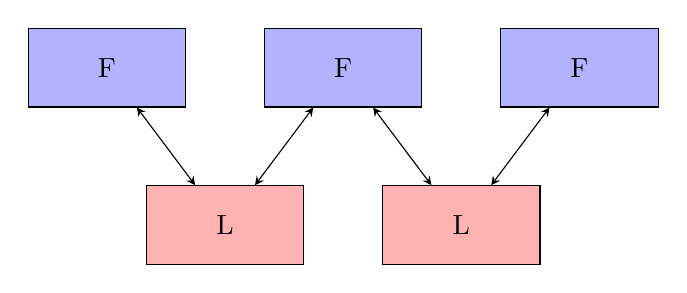
\begin{tikzpicture}
        \node[draw, rectangle, minimum width=2cm, minimum height=1cm, fill=blue!30] (F1) at (0,0) {F};
        \node[draw, rectangle, minimum width=2cm, minimum height=1cm, fill=blue!30] (F2) at (3,0) {F};
        \node[draw, rectangle, minimum width=2cm, minimum height=1cm, fill=blue!30] (F3) at (6,0) {F};
        \node[draw, rectangle, minimum width=2cm, minimum height=1cm, fill=red!30] (L1) at (1.5,-2) {L};
        \node[draw, rectangle, minimum width=2cm, minimum height=1cm, fill=red!30] (L2) at (4.5,-2) {L};

        \draw[<->, >=stealth] (F1) -- (L1);
        \draw[<->, >=stealth] (F2) -- (L1);
        \draw[<->, >=stealth] (F2) -- (L2);
        \draw[<->, >=stealth] (F3) -- (L2);
    \end{tikzpicture}
    \caption{Full nodes and lightweight nodes in a blockchain network}
    \label{fig:nodes}
\end{figure}

Figure \ref{fig:nodes} illustrates the interaction between full nodes and lightweight nodes in a blockchain network. In this example, lightweight nodes (L) communicate with full nodes (F) to request and verify specific parts of the blockchain. Full nodes are responsible for maintaining the complete blockchain data and ensuring the security and decentralization of the network. Lightweight nodes, on the other hand, provide a more accessible entry point for users with limited resources or network connectivity, allowing them to participate in the blockchain network without needing to store the entire blockchain.

\subsubsection{Mining and Consensus}
Mining is the process of validating and adding new transactions to the blockchain \cite{antonopoulos2014mastering}. Miners compete to solve a cryptographic puzzle, which requires substantial computational power. This process is energy-intensive and is known as Proof of Work (PoW) \cite{nakamoto2008bitcoin}. The first miner to solve the puzzle adds the new block to the chain and receives a reward in the form of newly minted bitcoins. This process serves as the consensus mechanism for the Bitcoin blockchain, ensuring that the blockchain is secure, resistant to tampering, and that all nodes agree on the state of the network \cite{swan2015blockchain}.


\begin{figure}[ht]
\centering
\begin{tikzpicture}[
    block/.style={rectangle, draw, text centered, rounded corners, minimum height=2em},
    arrow/.style={thick,->,>=stealth}
]
\node[block] (transactions) {New Transactions};
\node[block, below=1cm of transactions] (unconfirmed) {Unconfirmed Transactions};
\node[block, below=1cm of unconfirmed] (candidate) {Candidate Block};
\node[block, below=1cm of candidate] (puzzle) {Solve Puzzle (PoW)};
\node[block, below=2cm of puzzle] (mined) {Mined Block};
\node[block, left=1cm of mined] (previous) {Previous Block};

\draw[arrow] (transactions) -- (unconfirmed);
\draw[arrow] (unconfirmed) -- (candidate);
\draw[arrow] (candidate) -- (puzzle);
\draw[arrow] (puzzle) -- node[right, font=\small] {Valid Solution} (mined);
\draw[arrow] (previous) -- (mined);

\end{tikzpicture}
\caption{Mining process in Bitcoin.}
\label{fig:mining_process}
\end{figure}

Figure \ref{fig:mining_process} illustrates the mining process in Bitcoin. Miners collect new transactions from the network and assemble them into a block. They then perform a hash operation on the block header, which includes the hash of the previous block, a timestamp, a nonce, and a Merkle root representing the transactions in the block. The goal of the miner is to find a nonce that produces a hash value lower than a specific target set by the network difficulty. This process is computationally expensive, and miners often need to try billions of nonce values before finding a valid solution.

Once a miner finds a valid nonce, it broadcasts the solved block to the network. Other nodes verify the block's validity by checking if the hash meets the target difficulty and if the transactions in the block are valid. If the block is valid, the nodes update their local copy of the blockchain and begin mining the next block.

The PoW consensus mechanism makes it extremely difficult for an attacker to tamper with the blockchain. An attacker would need to control more than 50\% of the network's mining power to successfully launch a 51\% attack and modify the blockchain. This level of control is unlikely and economically infeasible due to the vast number of miners and the significant computational resources required for mining.

\begin{lstlisting}[language=Python, caption={Proof of Work Mining Process}, label={lst:pow_mining}]
import hashlib
import time

class ProofOfWork:
    def __init__(self, difficulty):
        self.difficulty = difficulty

    def mine(self, block):
        while True:
            block.nonce += 1
            hash_value = self.calculate_hash(block)
            if self.is_valid(hash_value):
                block.hash = hash_value
                return block

    def calculate_hash(self, block):
        block_data = str(block.prev_hash) + str(block.timestamp) + str(block.data) + str(block.nonce)
        return hashlib.sha256(block_data.encode('utf-8')).hexdigest()

    def is_valid(self, hash_value):
        target = '0' * self.difficulty
        return hash_value.startswith(target)

class Block:
    def __init__(self, prev_hash, data):
        self.prev_hash = prev_hash
        self.timestamp = int(time.time())
        self.data = data
        self.nonce = 0
        self.hash = ""

# Example usage:
difficulty = 4
pow = ProofOfWork(difficulty)

genesis_block = Block("0", "Genesis Block")
mined_genesis_block = pow.mine(genesis_block)

print("Mined Genesis Block:")
print("Nonce:", mined_genesis_block.nonce)
print("Hash:", mined_genesis_block.hash)
\end{lstlisting}

This example demonstrates a simple implementation of the Proof of Work mining process in Python. The \texttt{ProofOfWork} class takes a \texttt{difficulty} parameter, which determines the number of leading zeros required in the hash value. The \texttt{mine} function iterates through different nonce values until a hash meeting the difficulty requirement is found.

In the example usage, a genesis block is created and mined using the Proof of Work algorithm with a specified difficulty. The mined block's nonce and hash values are then printed.

\subsection{Types of Blockchain}
\label{sec:types_of_blockchain}

There are three primary types of blockchains:

\begin{enumerate}
    \item \textbf{Public Blockchains:} Public blockchains are open to anyone, allowing users to participate in the network without any restrictions. Examples include \ac{BTC}\cite{nakamoto2008bitcoin} and \ac{Ethereum}\cite{wood2014ethereum}.
    
    \item \textbf{Private Blockchains:} Private blockchains restrict participation to a selected group of users, typically within a single organization. These blockchains offer greater control over the network and its participants but sacrifice decentralization.
    
    \item \textbf{Consortium Blockchains:} Consortium blockchains are governed by a group of organizations that collectively manage the network. They offer a balance between the openness of public blockchains and the control of private blockchains. An example is Hedera Hashgraph.
\end{enumerate}

\subsection{Consensus Mechanisms}
\label{sec:consensus_mechanisms}

Consensus mechanisms are algorithms that enable blockchain networks to reach agreement on the state of the shared ledger. They ensure that all participants follow the same set of rules and prevent malicious actors from taking control of the network. Two of the most widely used consensus mechanisms are Proof of Work (PoW) and Proof of Stake (PoS).

\subsubsection{Proof of Work (PoW)}
\label{sec:proof_of_work}

Proof of Work (PoW) is the consensus mechanism used by Bitcoin\cite{nakamoto2008bitcoin} and other cryptocurrencies. In PoW, network participants called miners compete to solve complex mathematical puzzles in order to validate transactions and add new blocks to the blockchain. The first miner to solve the puzzle is rewarded with newly minted cryptocurrency. PoW provides strong security guarantees but can be energy-intensive and may lead to centralization as mining becomes more specialized and concentrated.

\subsubsection{Proof of Stake (PoS)}
\label{sec:proof_of_stake}

Proof of Stake (PoS) is an alternative consensus mechanism that aims to address some of the limitations of PoW. In PoS, validators are chosen to create new blocks and validate transactions based on their stake, or the amount of cryptocurrency they hold and are willing to lock as collateral. Validators are rewarded with transaction fees and may also receive newly minted cryptocurrency. PoS is more energy-efficient than PoW and can provide a more decentralized network, as it encourages participation from a larger number of validators. Ethereum currently transitioned from PoW to PoS with its Ethereum 2.0 upgrade\cite{buterin2013ethereum}.

\subsection{The Blockchain Trilemma}
The blockchain trilemma is a concept introduced by Ethereum co-founder Vitalik Buterin to describe the challenge of achieving three desirable characteristics in a blockchain system: decentralization, security, and scalability \cite{buterin2016impossible}. According to the trilemma, it is difficult to achieve all three properties simultaneously, and compromises must be made to optimize the performance of the system.

\begin{itemize}
\item \textbf{Decentralization} refers to the distribution of control and decision-making power within the network. A decentralized system is more resistant to censorship and single points of failure. Decentralization is achieved through consensus mechanisms and the use of a distributed network of nodes.
\item \textbf{Security} encompasses the protection of the system against attacks, data manipulation, and other forms of malicious behavior. A secure blockchain is resistant to various attack vectors, such as double-spending, Sybil attacks, and 51\% attacks. Security is usually maintained through cryptographic techniques, economic incentives, and robust consensus mechanisms.

\item \textbf{Scalability} refers to the ability of the system to handle an increasing number of transactions and participants without significant performance degradation. A scalable blockchain can support a growing user base and increasing transaction volumes. Scalability is often achieved by optimizing transaction processing and data storage.
\end{itemize}

The blockchain trilemma suggests that improving one aspect of the system may come at the cost of the other two. For example, increasing decentralization could lead to reduced scalability due to increased data replication and communication overhead. Similarly, improving scalability may require sacrificing decentralization or security.

Various solutions have been proposed to address the trilemma, such as sharding, off-chain scaling solutions (e.g., layer 2 protocols like the Lightning Network or xDai), and alternative consensus mechanisms. However, finding the optimal balance between these three properties remains an ongoing challenge in the development of blockchain technology.

\section{Ethereum}
Ethereum is a public, open-source, decentralised platform that runs smart contracts: applications that execute precisely as programmed without any possibility of fraud or third-party interference \cite{buterin2013ethereum}. The platform comprises two core components: Ethereum's blockchain and the Ethereum Virtual Machine (EVM), which operates on the Ethereum network. The Ethereum blockchain is a global, decentralised computer capable of executing code as programmed, while the EVM is a virtual machine that runs smart contracts on the Ethereum network \cite{wood2014ethereum}.

Ethereum expands the capabilities of traditional blockchains like Bitcoin by enabling developers to create decentralised applications (dApps) and smart contracts \cite{swan2015blockchain}. These applications operate on the Ethereum network and are generally open-source and decentralised. Furthermore, Ethereum facilitates the creation of decentralised autonomous organisations (DAOs) \cite{mougayar2016business}.

In Ethereum, transactions and contract executions require "gas" fees to prevent spam and allocate resources on the network. Gas fees are paid in Ether (ETH), the native cryptocurrency of the Ethereum network \cite{antonopoulos2018mastering}.

\subsection{Computation And Turing-Complete}
A Turing-complete system can perform any computation with enough time and resources \cite{turing1936computable}. Ethereum, with its Ethereum Virtual Machine (EVM), is Turing-complete, which means it can execute any arbitrary algorithm if sufficient resources are available \cite{buterin2013ethereum}. This capability allows developers to create diverse applications and smart contracts on the Ethereum platform, making it more versatile than more straightforward, non-Turing-complete blockchains like Bitcoin.

\subsection{Smart Contracts}
Smart contracts are self-executing contracts with the terms of the agreement between parties directly written into lines of code \cite{szabo1997formalizing}. They facilitate, verify, or enforce the negotiation or performance of a contract, allowing credible transactions without third parties. These transactions are trackable and irreversible \cite{kosba2016hawk}.

Smart contracts were popularized with the introduction of the Ethereum blockchain, which extended the capabilities of \ac{BTC} by adding a more expressive and flexible programming language, called Solidity, for contract development. Smart contracts run on the Ethereum platform, enabling various use cases, such as token creation, decentralized finance (DeFi), and decentralized applications (dApps) \cite{mougayar2016business2}.

\subsubsection{How Smart Contracts Work}
Smart contracts work by using blockchain technology to store and execute predefined rules. When certain conditions encoded in the smart contract are met, it triggers the execution of specific actions. These actions can include transferring tokens, updating the state of the contract, or calling other smart contracts. Smart contracts are tamper-proof, transparent, and autonomous, ensuring that the agreed-upon terms are executed without the need for intermediaries.

Smart contracts are executed in a decentralized manner by every node participating in the blockchain network. Each node runs the same code and independently validates the results, ensuring consensus and trust in the execution of the contract.

\subsubsection{Components of a Smart Contract}
A smart contract typically consists of the following components:

\begin{itemize}
    \item \textbf{Contract Creator}: The contract creator creates the contract and sets the conditions.
    \item \textbf{Signatories}: The parties that agree to the terms of the contract.
    \item \textbf{Conditions}: The rules that the signatories must follow.
    \item \textbf{Actions}: The tasks that the signatories must perform.
    \item \textbf{Variables}: These store the state of the contract, such as account balances or other data. Variables can be of different data types, such as integers, strings, or custom-defined data structures.
    \item \textbf{Functions}: Functions define the contract's behavior and can be called by external users or other smart contracts. They can read and modify the contract's state, interact with other contracts, or emit events. Functions can have visibility modifiers, such as public, private, or internal, which determine who can call the function.
    \item \textbf{Events}: Events are used to notify external parties about changes in the contract's state or the occurrence of specific actions. They are logged on the blockchain and can be queried by external applications, such as user interfaces or other smart contracts.
    \item \textbf{Modifiers}: Modifiers are used to modify the behavior of functions, often used for access control or precondition checks. They can enforce specific requirements that must be met before the function can be executed, such as checking whether the sender of a transaction has the necessary privileges or ensuring that a certain condition is true.
\end{itemize}

Here is a simple example of a Solidity smart contract that demonstrates some of these components:

\begin{lstlisting}[language=Java, caption={Smart Contract Template}, label={lst:sc_template}]
pragma solidity ^0.8.0;

contract SimpleBank {
    address public owner;
    mapping(address => uint256) private balances;
    event Deposit(address indexed sender, uint256 amount);
    event Withdrawal(address indexed recipient, uint256 amount);
    
    modifier onlyOwner() {
        require(msg.sender == owner, "Only the owner can call this function.");
        _;
    }
    
    constructor() {
        owner = msg.sender;
    }
    
    function deposit() public payable {
        balances[msg.sender] += msg.value;
        emit Deposit(msg.sender, msg.value);
    }
    
    function withdraw(uint256 amount) public {
        require(balances[msg.sender] >= amount, "Insufficient balance.");
        balances[msg.sender] -= amount;
        payable(msg.sender).transfer(amount);
        emit Withdrawal(msg.sender, amount);
    }
    
    function getBalance() public view returns (uint256) {
        return balances[msg.sender];
    }
    
    function transferOwnership(address newOwner) public onlyOwner {
        owner = newOwner;
    }
}
\end{lstlisting}

Smart contracts are executed within the \ac{EVM}, a runtime environment for executing Turing-complete code on the Ethereum blockchain. The \ac{EVM} isolates smart contracts from the underlying hardware and operating system, providing a secure and consistent execution environment.

\subsubsection{Ethereum Virtual Machine}
The Ethereum Virtual Machine (EVM) is a decentralized virtual machine that runs Turing-complete smart contracts on the Ethereum blockchain \cite{wood2014ethereum}. The EVM ensures that smart contracts are executed in a secure and isolated environment, free from interference from the underlying hardware or operating system \cite{buterin2013ethereum}.

Some key features of the EVM include:

\begin{itemize}
\item \textbf{Isolation}: Each smart contract runs in its own isolated environment, preventing unauthorized access to other smart contracts or the underlying system.
\item \textbf{Turing-complete}: The EVM supports a Turing-complete instruction set, which means it can execute any algorithm, given enough resources.
\item \textbf{Deterministic}: The execution of a smart contract is deterministic, meaning that given the same input, it will always produce the same output.
\item \textbf{Sandboxed}: The EVM is sandboxed, which means that the smart contract code is restricted from accessing resources outside its own environment, ensuring security and integrity.
\end{itemize}

\subsection{Fees}
In blockchain networks, fees are typically required for various transactions and operations. These fees serve as an incentive for the network's miners or validators to process and validate transactions, as well as a mechanism to prevent spam and malicious activity. In Ethereum, fees are called "gas," and they are paid in the native cryptocurrency Ether (ETH) \cite{wood2014ethereum}. Gas fees are determined by the complexity of the transaction or operation, and they can fluctuate based on network congestion and demand. As a result, users need to consider the gas fees when interacting with the Ethereum network, especially when executing smart contracts or participating in decentralised applications \cite{wood2014ethereum}.

\subsubsection{Gas}
Gas is a unit of measure used to quantify the computational work required to execute operations in the EVM \cite{wood2014ethereum}. Each opcode (operation code) in the EVM has a specific gas cost associated with it. The sender of a transaction must pay for the gas consumed by their transaction in Ether, which is then awarded to the miner who includes the transaction in a block.

Some key aspects of gas include:

\begin{itemize}
    \item \textbf{Resource Limitation}: Gas serves as a mechanism to limit the resources consumed by smart contracts, preventing infinite loops or excessive computation.
    \item \textbf{Incentivization}: By charging users for the computational resources their transactions consume, gas provides an incentive for miners to validate and include transactions in blocks.
    \item \textbf{Dynamic Pricing}: Users can specify the gas price they are willing to pay for their
\end{itemize}

\subsection{Solidity}
Solidity is a high-level, statically-typed programming language designed specifically for developing smart contracts on the Ethereum blockchain \cite{solidityDocs}. It was proposed by Gavin Wood \cite{wood2014ethereum} and developed by the Ethereum team in 2014. Solidity has a syntax that is similar to JavaScript, making it easier for developers to learn and adopt \cite{antonopoulos2018mastering}.

Smart contracts written in Solidity are compiled into bytecode, which can be executed on the Ethereum Virtual Machine (EVM) \cite{wood2014ethereum}. Solidity supports inheritance, libraries, and complex user-defined types, enabling the creation of sophisticated and modular smart contracts \cite{antonopoulos2018mastering}.

Some key features of Solidity include:
\begin{itemize}
\item \textbf{Type-safe language:} Solidity is a statically-typed language, which helps prevent common programming errors by enforcing type checking at compile-time \cite{solidityDocs}.
\item \textbf{Contract-oriented:} Solidity is designed specifically for writing smart contracts, with built-in support for contract-related features like state variables, functions, and events \cite{solidityDocs}.
\item \textbf{Ethereum integration:} Solidity smart contracts can interact with Ethereum's native cryptocurrency, Ether (ETH), and other tokens built on the platform \cite{wood2014ethereum}.
\end{itemize}

Solidity has undergone continuous development and improvements, with multiple versions being released since its inception. It has become the de facto language for writing smart contracts on the Ethereum platform and is widely used in the blockchain development community \cite{antonopoulos2018mastering}.

\subsection{Scaling and Layer Solutions}
Blockchain scalability is a crucial aspect to achieve widespread adoption and efficient operation. As a result, several scaling and layer solutions have been developed to improve the performance of blockchains \cite{pisa2019state, buterin2018layer2}.

\subsubsection{Layer 1}
Layer 1, also known as the base layer, refers to the core blockchain protocol itself. In the context of Ethereum, Layer 1 comprises the Ethereum blockchain and its consensus mechanism, smart contract functionality, and native token (Ether). Optimizations at the base layer aim to improve the underlying blockchain protocol by increasing transaction throughput, reducing fees, and enhancing security \cite{wood2014ethereum}.

\subsubsection{Layer 2}
Layer 2 solutions are built on top of the base layer (Layer 1) and aim to improve the blockchain's scalability, speed, and efficiency without modifying the underlying protocol. Examples of Layer 2 solutions include sidechains, state channels, and rollups \cite{buterin2018layer2}. These solutions enable off-chain transactions and computation, thus reducing the load on the main blockchain, improving transaction throughput, and decreasing fees. The results of these off-chain operations are then securely transferred back to the main blockchain, leveraging the security and decentralization of Layer 1 \cite{pisa2019state}.

\subsubsection{Gnosis Chain}
Gnosis Chain, formerly known as xDai Chain, is a Layer 2 solution for Ethereum that utilizes a Proof-of-Stake consensus mechanism. It is an EVM-compatible sidechain designed for fast and low-cost transactions \cite{gnosischain}. Gnosis Chain is built on the Gnosis Protocol, which allows for decentralized finance (DeFi) applications and prediction markets. The native token of Gnosis Chain is the GNO token, which is used for transaction fees and staking \cite{gnosischain}.

\subsection{Tokens}
Tokens are digital assets on a blockchain network and can represent various types of value. They can be fungible, meaning they are interchangeable and have the same value, like a digital currency, or non-fungible, meaning they are unique and cannot be exchanged on a one-to-one basis, like digital collectables. Ethereum is a popular platform for creating and managing tokens due to its support for smart contracts and various token standards \cite{vogelsteller2015erc20}.

\subsubsection{Non-Fungible}
\ac{NFT}s are unique, indivisible digital assets that cannot be exchanged on a one-to-one basis with other tokens. \ac{NFT}s can represent digital art, collectables, virtual real estate, and other valuable digital assets. Unlike fungible tokens, where each unit is interchangeable and has the same value, non-fungible tokens have distinct properties that make them unique and valuable in their own right \cite{entriken2018erc721}. \ac{NFT}s are commonly used for digital art and collectables, and they have gained significant attention due to high-profile sales and celebrity endorsements. Ethereum is the primary platform for creating and trading \ac{NFT}s due to its support for various token standards, such as ERC-721 and ERC-1155, which enable the creation and management of non-fungible tokens.

\subsubsection{ERC-721}
ERC-721 is a widely adopted Ethereum token standard for non-fungible tokens. It defines a set of rules and functions that enable creating, managing, and transferring unique tokens on the Ethereum blockchain \cite{entriken2018erc721}. ERC-721 tokens can represent digital assets such as digital art, virtual goods, and collectables. The standard has gained popularity due to its ability to provide a robust framework for creating unique tokens with individual attributes and provenance information \cite{entriken2018erc721}. This standard has been instrumental in the growth of the \ac{NFT} market, as it allows developers to build and deploy smart contracts that manage non-fungible tokens, enabling a wide range of applications and use cases in the digital asset space.

\subsubsection{POAP}
Proof of Attendance Protocol (POAP) is a decentralized protocol built on the Ethereum blockchain that enables the creation and distribution of unique digital tokens, called POAP tokens, as proof of attendance or participation in events, conferences, or other activities \cite{poapWebsite}. These tokens are non-fungible and can be collected, traded, or used as access keys for special events or rewards.

POAP tokens are ERC-721 compliant, which means they follow the Ethereum standard for non-fungible tokens (\ac{NFT}s). Each POAP token is unique and has a distinct identifier, metadata, and graphic design, representing the specific event or activity it was issued for \cite{poapGithub}.

The POAP ecosystem consists of various components, including a minting platform for event organizers to create and distribute tokens, a mobile app and web application for users to manage and display their collection of tokens, and an API for developers to build and integrate new applications and services using POAP tokens \cite{poapWebsite}. You can see the smart contract in Figure \ref{sc:poapContract}


\subsubsection{ERC-1155}
ERC-1155 is an Ethereum token standard that extends the functionality of ERC-721 and ERC-20, allowing for the creation and management of both fungible and non-fungible tokens within a single, smart contract \cite{vogelsteller2015erc20}. This standard enables greater efficiency and flexibility in token management, reducing the need for deploying multiple contracts for different types of tokens. ERC-1155 tokens can represent various digital assets, including gaming items, digital art, and collectables, and can be traded on marketplaces that support the standard \cite{openzeppelinerc1155}. By allowing developers to create and manage multiple token types within a single contract, ERC-1155 optimises the process. It reduces the gas fees associated with token transactions, making it an attractive option for projects that require a diverse range of digital assets.

\subsubsection{Fungible}
Fungible tokens are a type of cryptographic token that are interchangeable with one another, meaning that each token is identical in specification and value \cite{vogelsteller2015erc20}. This characteristic enables fungible tokens to be used as a medium of exchange, as they can be easily exchanged for an equal quantity of the same token. These tokens are commonly used for various purposes, such as representing currencies, points, or rewards in a digital ecosystem. Fungible tokens are often built on platforms like Ethereum, which support the creation and management of tokens using well-established token standards such as ERC-20.

\subsubsection{ERC-20}
ERC-20 is a widely adopted token standard on the Ethereum blockchain for creating and issuing fungible tokens \cite{vogelsteller2015erc20}. The ERC-20 standard establishes a common set of rules and functions for token contracts, allowing developers to create easily compatible tokens with other ERC-20-compliant applications, such as wallets and decentralised exchanges.

The ERC-20 standard defines a set of six functions and two events that a token contract must implement. These functions and events enable developers to manage token transactions, query the balance of an account, and transfer tokens between accounts.

Some of the critical functions specified in the ERC-20 standard include:
\begin{enumerate}
\item	\textbf{totalSupply:} Returns the total number of tokens in circulation.
\item	\textbf{balanceOf:} Returns the token balance of a specified address.
\item	\textbf{transfer:} Transfers a specific amount of tokens from the sender's address to a recipient's address.
\item	\textbf{approve:} Allows the owner of an address to authorize a third party to spend a specific amount of tokens on their behalf.
\item	\textbf{allowance:} Returns the number of tokens a third party can spend on behalf of a specified address.
\item	\textbf{transferFrom:} Allows a third party to transfer tokens from one address to another, provided they have been granted approval.
\end{enumerate}

The widespread adoption of the ERC-20 standard has led to increased interoperability and ease of use within the Ethereum ecosystem, facilitating the development and deployment of various decentralized applications that utilize fungible tokens \cite{vogelsteller2015erc20}. As a foundational standard, ERC-20 has also inspired the creation of other token standards, such as ERC-721 for non-fungible tokens (NFTs) \cite{entriken2018erc721} and ERC-1155 for multi-token contracts \cite{eip2018eip1155}. These subsequent standards build upon the principles and functionalities of ERC-20 while introducing new features and use cases for tokenized assets on the Ethereum blockchain.

\section{Zero-Knowledge Proof}
In cryptography, a zero-knowledge proof (ZKP) or zero-knowledge protocol is a method by which one party (the prover) can prove to another party (the verifier) that they know a value x without conveying any information about what that value is. The essence of zero-knowledge proofs is that it is trivial to prove that one possesses knowledge of certain information by simply revealing it; the challenge is to prove such knowledge without revealing the information itself or any additional information \cite{goldreich1986proofs}.

ZKPs must satisfy the following properties. The first is completeness, where the prover can convince the verifier if given a true statement. The second is soundness, where a false statement cannot convince a verifier that a malicious prover was sent. Finally, zero-knowledge, in which the statement is true or false, is the only information revealed and nothing else.

Zero-knowledge proofs are often used in conjunction with cryptographic protocols to ensure no leaking of certain information during the execution of the protocol. They have gained significant attention in recent years, particularly in the context of blockchain technology and privacy-preserving applications \cite{bensasson2014zerocash}.

To illustrate the concept of zero-knowledge proofs, let's consider a simple example: the Ali Baba's cave scenario. In this scenario, the prover (Peggy) wants to convince the verifier (Victor) that she knows the secret password to open a door in the cave without revealing the password itself. The cave is in the shape of a rectangular loop with the door separating the two halves of the cave (see Figure \ref{fig:rectangles_t}).

\begin{figure}[h]
\centering
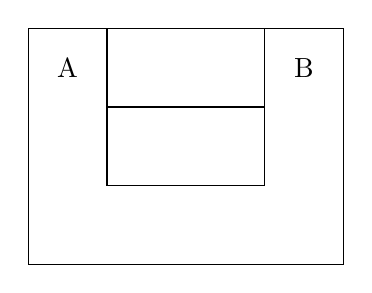
\begin{tikzpicture}
    % Outer rectangle
    \draw (0,0) rectangle (4,3);
    % Inner rectangle
    \draw (1,1) rectangle (3,2);
    % Horizontal rectangle
    \draw (1,2) rectangle (3,3);
    \node at (0.5,2.5) {A};
    \node at (3.5,2.5) {B};
\end{tikzpicture}
\caption{Representation of Ali Baba's cave with the door separating parts A and B.}
\label{fig:rectangles_t}
\end{figure}

The protocol proceeds as follows:

\begin{enumerate}
    \item Victor waits outside while Peggy enters the cave through either part A or B.
    \item Victor enters the cave and shouts which side Peggy should come out from (either A or B).
    \item Peggy uses the secret password to open the door, if necessary, and comes out of the requested side.
\end{enumerate}

This process is repeated multiple times. If Peggy knows the password, she can always come out from the requested side. If she does not know the password, she has a 50\% chance of guessing Victor's request correctly in each iteration. After $n$ iterations, the probability that Peggy is guessing correctly each time is $1/2^n$.


\subsection{Non-interactive zero-knowledge proofs}
Non-interactive zero-knowledge proofs (NIZK) are a type of zero-knowledge proof in which the interaction between the prover and the verifier is limited to a single message from the prover to the verifier. In contrast to interactive zero-knowledge proofs, where the prover and verifier engage in multiple rounds of communication, NIZK proofs do not require any back-and-forth communication between the parties \cite{blum1988noninteractive}. This property makes NIZK proofs particularly well-suited for applications where communication is limited or expensive, such as blockchain networks and secure messaging systems.

\subsection{ZK-SNARKs}
Zero-Knowledge Succinct Non-Interactive Argument of Knowledge (ZK-SNARK) is a type of non-interactive zero-knowledge proof that allows a prover to demonstrate the validity of a statement succinctly and efficiently. ZK-SNARKs have gained significant attention in blockchain technology due to their ability to provide privacy and scalability \cite{bensasson2013snarks}.

The term "succinct" refers to the fact that ZK-SNARK proofs are small and can be verified quickly, making them practical for real-world applications. ZK-SNARKs achieve this efficiency through advanced cryptographic techniques, such as elliptic curve pairings and homomorphic encryption \cite{groth2016size}.

One of the primary applications of ZK-SNARKs is in privacy-preserving cryptocurrencies, such as Zcash, which uses ZK-SNARKs to enable private transactions. With ZK-SNARKs, users can prove that they possess the necessary funds to perform a transaction without revealing the actual amounts or addresses involved, thereby maintaining the privacy of the users and the transaction details \cite{hopwood2020zcash}.

Additionally, ZK-SNARKs can improve the scalability of blockchain networks by offloading complex computations off-chain and providing a succinct proof that can be verified on-chain. This reduces the burden on the network, allowing for more efficient processing of transactions \cite{bensasson2019scalable}.

\subsection{ZK-STARKs}
Zero-Knowledge Scalable Transparent ARguments of Knowledge (ZK-STARK) is another type of non-interactive zero-knowledge proof that offers many of the benefits of ZK-SNARKs but with added transparency and post-quantum security \cite{bensasson2019aurora}. Unlike ZK-SNARKs, which rely on a trusted setup phase and utilise cryptographic assumptions that may be vulnerable to quantum computers, ZK-STARKs are based on more conservative cryptographic assumptions and do not require a trusted setup.

ZK-STARKs use a combination of error-correcting codes, hash functions, and interactive oracle proofs to create a succinct and efficient proof system. The main advantage of ZK-STARKs over ZK-SNARKs is their transparency. They do not rely on a trusted setup, eliminating the need for a common reference string and reducing the potential for manipulation or collusion \cite{bensasson2018scalable}.

Another advantage of ZK-STARKs is their resistance to quantum attacks, making them a more future-proof solution for privacy and scalability in the context of blockchain technology and other cryptographic applications. However, ZK-STARK proofs are typically more extensive and more computationally intensive to generate than ZK-SNARK proofs, which can be a trade-off for some applications \cite{bensasson2020primer}.

ZK-STARKs have potential use cases in various industries, including finance, healthcare, and supply chain management, where privacy and data integrity are paramount. They are also being researched for their potential to improve the scalability and privacy of blockchain networks, similar to ZK-SNARKs \cite{maller2019sonic}.

\subsubsection{Semaphores}
In the context of zero-knowledge proofs and cryptography, Semaphores refer to a privacy-preserving signalling mechanism that enables users to prove membership in a group without revealing their identity \cite{bunz2018bulletproofs}. Semaphores utilise zero-knowledge proofs to maintain the anonymity of users while allowing them to prove that they belong to a specific group or set. This enables various applications, such as anonymous voting systems, secure messaging, and privacy-preserving authentication.

Semaphore constructions typically involve Merkle trees and zero-knowledge proof systems like ZK-SNARKs or ZK-STARKs. A group administrator generates a Merkle tree with the public keys of all group members, and each member receives their corresponding Merkle proof. To signal their membership, a user generates a zero-knowledge proof that attests to possessing a valid Merkle proof without revealing the specific public key or identity \cite{idrees2019zkay}.

The Semaphore construction ensures that only authorised users can generate valid proofs, preventing unauthorized users from pretending to be part of the group. Moreover, the zero-knowledge aspect of Semaphore ensures that the user's identity remains hidden, providing strong privacy guarantees.

Semaphores have potential applications in various domains where privacy and authentication are crucial, such as secure voting systems, whistleblowing platforms, and anonymous credential systems \cite{benarroch2020improved}.

\subsubsection{Circoms}
Circom is a domain-specific language (DSL) and compiler for creating arithmetic circuits \cite{jorda2019circom}. These circuits are essential for constructing zero-knowledge proofs, as they allow developers to create complex cryptographic proofs without an in-depth understanding of the underlying mathematics. Circom enables developers to write human-readable code for arithmetic circuits, which is then compiled into a more efficient representation that can be used with various zero-knowledge proof systems, such as ZK-SNARKs and ZK-STARKs.

Circom simplifies creating circuits by allowing developers to use familiar programming constructs, such as loops and conditionals, while automatically handling low-level circuit optimisations. The resulting circuits can be used to create and verify zero-knowledge proofs that attest to the correctness of specific statements without revealing any underlying information. This functionality has been used in various applications, including privacy-preserving smart contracts, anonymous voting systems, and confidential asset transfers \cite{maller2019sonic2}.

